\section{The Games on Track GT-position system}
The Games on Track GT-Position system, shortened GoT, is a GPS system which uses radio-waves and ultrasound to locate the object. The system is build up by three hardware components, the transmitter, receiver and master. 

\subsubsection{Transmitter}
The transmitter component is placed on the object, which needs to be located. To indicate the objects position, the transmitters emits out ultrasound waves to indicate where it and the object is positioned. The transmitter component runs on 2 AA-batteries and therefore does not need an external power-source. 

\subsubsection{Receiver}
\todo{What kind of "radio waves" does the receiver transmit data to the master?}
The receiver component is placed around the area where the object, with the transmitter, has to be located. The receivers assignment is to search for the ultrasound waves, which the transmitter is emitting. The ultrasound waves received by the receivers, provides information containing the distance between the specific receiver to the transmitter located on the object. To be able to calculate the exact position of the transmitter and the object, a minimum of three receivers is necessary. however, more receivers can be added to the system for more reliability and the ability to cover a larger area. For the receivers to work at a high efficiency, they should be placed 1 to 2 meters apart and not on a single line. But if receivers shall cover a bigger area, they can be placed up to a distance of 5 meters between them, however, this would affect the measurement and thereby make it less reliable. Each receiver have a maximum range of 8 meters and as seen on \figref{receiverSetup}, the three receivers should be placed in each others reach. The receivers needs between 14 to 20 volt DC. Thus, making the receivers able to be powered through a computer charger if necessary.

\begin{figure}[H]
	\centering
	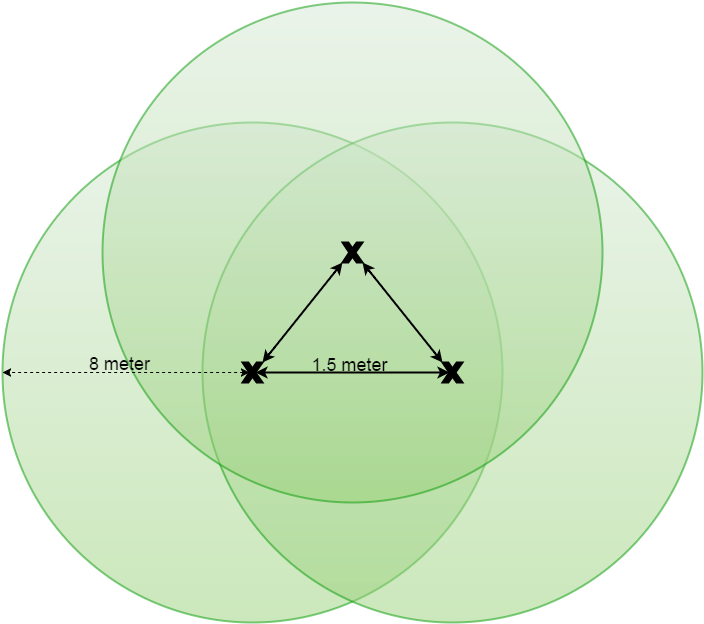
\includegraphics[scale=0.5]{figures/ReceiverSetup.png}
	\caption{Example on a standard setup for the receivers (increase size of text in figure)}
	\label{receiverSetup}
\end{figure}

\subsubsection{Master}
The master is a receiver which should be connected to a computer. The masters assignment is to receive the data transmitted from the individual receivers and send it directly to the connected computer. The master is powered through a USB cable, between the master and the computer.
\subsubsection{Computer}

The program on the computer, which handles the information received from the master, uses the data to calculate the position of the transmitter. This is done with a method call Trilateration. Trilateration is a way of calculating a position, in a three-dimensional space, from three distances (from known locations), with the help of spheres, circles and triangles. Therefore it is necessary for the system to have atleast three receivers, as mentioned earlier. With additional receivers a check up can be performed to ensure the position of the transmitter is correct.\\\\

If the receivers have been moved, it is necessary to calibrate the system. This is done with a calibration triangle. The calibration triangle is three markings on the surface, that will be setup to be the zero surface for the Z-axis. One of the points on the calibration triangle is made the origin (0,0,0) of the coordinate system. Another point on the triangle will then be call (X,0,0), in which the line between the first point and the second point will become the X-axis. The last point will be call (X,Y,0) and will determine in which way the positive Y-axis will go. The surface which the calibration triangle is creating, will be the zero surface for the Z-axis, and is horizontal. The distance between the three points is measured and put into the software. Thereafter, with using the transmitter, are the position of the receivers calculated.  The transmitter is first placed in the first point (0,0,0), there next the second point (X,0,0) and then in the last point (X,Y,0). At each point the distance to the receivers is measured. Out from this data, about the placement of the points and their distance to the receivers, the software can calculate the position of each receiver, with the help of trilateration. \\\\

\todo{How should the recievers be placed? how far can they reach, picture?}

\todo{How do you calibrate, do you move the transmitter around?? but that in the text}

\todo{mergeconflict which needs to be addressed}

The program on the computer, which handles the information received from the master, uses the data to calculate the position of the transmitter. This is done with a method call Trilateration. Trilateration is a way of calculating a position, in a three-dimensional space, from three distances (from known locations), with the help of spheres, circles and triangles. Therefore it is necessary for the system to have atleast three receivers, as mentioned earlier.  With additional receivers a check up can be performed to ensure the position of the transmitter is correct. Trilateration does not work, if the three know points is on a single line and therefore shall the receivers be placed in a triangle.\\\\
\noindent
If the receivers have been moved, it is necessary to calibrate the system. This is done with a calibration triangle. The calibration triangle is made of three points on a flat surface and have a distance of 40 to 200 centimeters between them. One of the points on the calibration triangle is made the origin (0,0,0) of the new coordinate system. Another point on the triangle will then be call (X,0,0), in which the line between the first point and the second point will become the X-axis. The last point will be call (X,Y,0) and will determine in which way the positive Y-axis will go. The surface which the calibration triangle is placed on, will be the XY-plan, where Z will go positiv in the direction of the receivers. The distance between the three points is measured and put into the program. Thereafter, the transmitter placed in the three point, with (0,0,0) first and (X,Y,0) last. When the transmitter is placed in a point, the receivers measure the distance between them and the transmitter. From the data, the program can calculate the position of each receiver, with the help of trilateration. \\\\
